\documentclass[tikz,border=3pt]{standalone}
\usepackage{xcolor}
\usetikzlibrary{arrows.meta,calc}

% Shared with Fig. 1: geometry gray-blue, teal route, and warm semantic risk.
\definecolor{ink}{HTML}{24343D}
\definecolor{muted}{HTML}{657985}
\definecolor{rule}{HTML}{D9DEE3}
\definecolor{structure}{HTML}{657985}
\definecolor{candidate}{HTML}{B5C1C8}
\definecolor{depth}{HTML}{3973B7}
\definecolor{semantic}{HTML}{D14E46}
\definecolor{scorelow}{HTML}{EDF3F0}
\definecolor{scoremid}{HTML}{D9AD3D}
\definecolor{plan}{HTML}{007C83}
\definecolor{mission}{HTML}{C43C39}
\definecolor{frontier}{HTML}{E28A17}
\definecolor{localgoal}{HTML}{B64E8A}
\colorlet{structurebg}{structure!6}
\colorlet{depthbg}{depth!5}
\colorlet{semanticbg}{semantic!5}
\colorlet{planbg}{plan!5}

\begin{document}
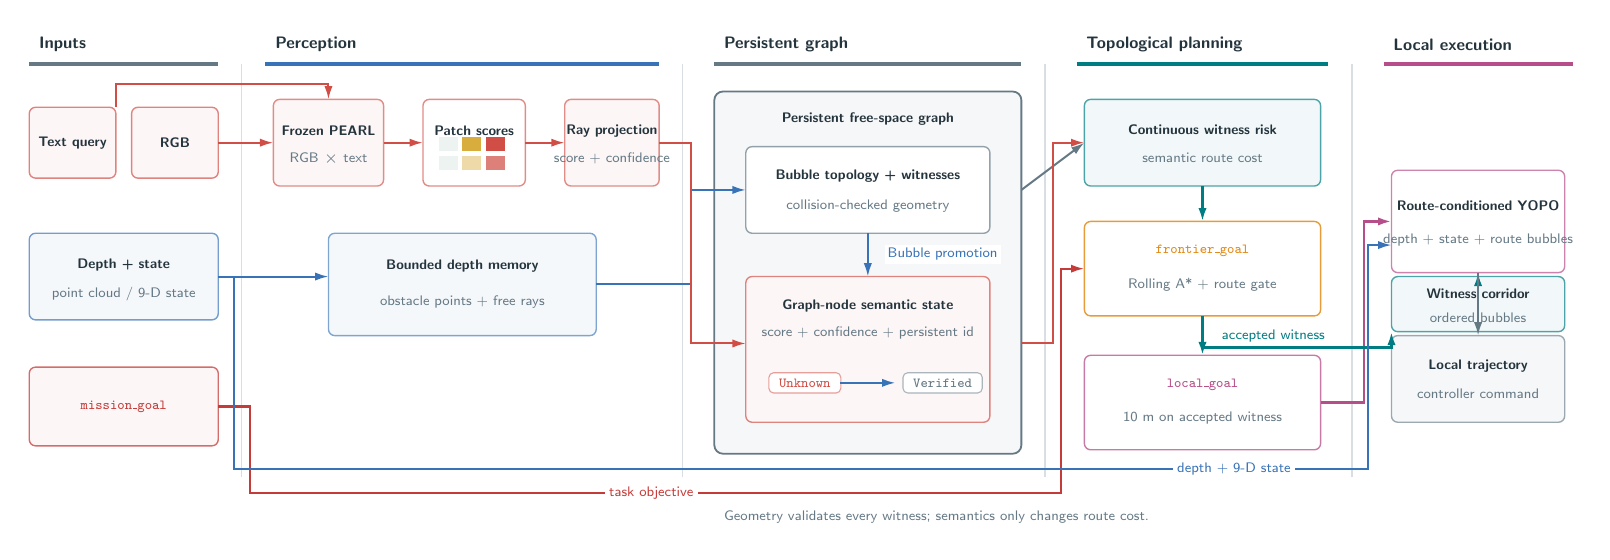
\begin{tikzpicture}[
  x=1mm,y=1mm,
  font=\sffamily,
  section/.style={font=\sffamily\bfseries\fontsize{6.4}{7.2}\selectfont,text=ink},
  box/.style={rounded corners=.8mm,line width=.5pt,fill=white,align=center,
              font=\sffamily\bfseries\fontsize{5.4}{6.2}\selectfont,text=ink},
  note/.style={font=\sffamily\fontsize{4.2}{4.9}\selectfont,text=muted,align=center},
  tag/.style={rounded corners=.6mm,inner xsep=1.3mm,inner ysep=.75mm,
              font=\ttfamily\bfseries\fontsize{4.5}{5.2}\selectfont},
  flow/.style={-{Latex[length=1.7mm,width=1.05mm]},line width=.72pt,draw=structure},
  semflow/.style={flow,draw=semantic},
  depthflow/.style={flow,draw=depth},
  planflow/.style={flow,draw=plan,line width=.9pt},
  localgoalflow/.style={flow,draw=localgoal,line width=.9pt},
  missionflow/.style={flow,draw=mission,line width=.78pt}
]

% Section headers and quiet separators.
\node[section,anchor=west] at (0,60) {Inputs};
\draw[structure,line width=1.15pt] (0,57.5)--(24,57.5);
\node[section,anchor=west] at (30,60) {Perception};
\draw[depth,line width=1.15pt] (30,57.5)--(80,57.5);
\node[section,anchor=west] at (87,60) {Persistent graph};
\draw[structure,line width=1.15pt] (87,57.5)--(126,57.5);
\node[section,anchor=west] at (133,60) {Topological planning};
\draw[plan,line width=1.15pt] (133,57.5)--(165,57.5);
\node[section,anchor=west] at (172,60) {Local execution};
\draw[localgoal,line width=1.15pt] (172,57.5)--(196,57.5);

\foreach \x in {27,83,129,168} {
  \draw[rule,line width=.45pt] (\x,5)--(\x,57.5);
}

% Inputs.
\filldraw[box,draw=semantic!70,fill=semanticbg] (0,43) rectangle (11,52);
\node[box,draw=none,fill=none] at (5.5,47.5) {Text query};
\filldraw[box,draw=semantic!70,fill=semanticbg] (13,43) rectangle (24,52);
\node[box,draw=none,fill=none] at (18.5,47.5) {RGB};

\filldraw[box,draw=depth!70,fill=depthbg] (0,25) rectangle (24,36);
\node[box,draw=none,fill=none] at (12,32) {Depth + state};
\node[note] at (12,28.3) {point cloud / 9-D state};

\filldraw[box,draw=mission!75,fill=semanticbg] (0,9) rectangle (24,19);
\node[tag,text=mission] at (12,14) {mission\_goal};

% Semantic and geometric perception lanes.
\filldraw[box,draw=semantic!65,fill=semanticbg] (31,42) rectangle (45,53);
\node[box,draw=none,fill=none] at (38,49) {Frozen PEARL};
\node[note] at (38,45.5) {RGB $\times$ text};

\filldraw[box,draw=semantic!65] (50,42) rectangle (63,53);
\node[box,draw=none,fill=none] at (56.5,49) {Patch scores};
\foreach \x/\y/\c in {52/44/scorelow,55/44/scoremid!45,58/44/semantic!72,
                         52/46.4/scorelow,55/46.4/scoremid,58/46.4/semantic} {
  \fill[\c] (\x,\y) rectangle ++(2.4,1.8);
}

\filldraw[box,draw=semantic!65,fill=semanticbg] (68,42) rectangle (80,53);
\node[box,draw=none,fill=none] at (74,49) {Ray projection};
\node[note] at (74,45.5) {score + confidence};

\draw[semflow] (24,47.5)--(31,47.5);
\draw[semflow] (11,52)--(11,55)--(38,55)--(38,53);
\draw[semflow] (45,47.5)--(50,47.5);
\draw[semflow] (63,47.5)--(68,47.5);

\filldraw[box,draw=depth!65,fill=depthbg] (38,23) rectangle (72,36);
\node[box,draw=none,fill=none] at (55,31.8) {Bounded depth memory};
\node[note] at (55,27.3) {obstacle points + free rays};
\draw[depthflow] (24,30.5)--(38,30.5);

% One persistent graph owns collision-checked geometry and semantic node state.
\filldraw[rounded corners=1.1mm,line width=.65pt,draw=structure,fill=structurebg]
  (87,8) rectangle (126,54);
\node[box,draw=none,fill=none] at (106.5,50.5) {Persistent free-space graph};

\filldraw[box,draw=structure!70,fill=white] (91,36) rectangle (122,47);
\node[box,draw=none,fill=none] at (106.5,43.3) {Bubble topology + witnesses};
\node[note] at (106.5,39.5) {collision-checked geometry};

\filldraw[box,draw=semantic!70,fill=semanticbg] (91,12) rectangle (122,30.5);
\node[box,draw=none,fill=none] at (106.5,26.8) {Graph-node semantic state};
\node[note] at (106.5,23.3) {score + confidence + persistent id};
\node[tag,text=semantic,draw=semantic!55,fill=white] at (98.5,17) {Unknown};
\draw[depthflow] (103,17)--(110,17);
\node[tag,text=structure,draw=structure!55,fill=white] at (116,17) {Verified};

\draw[depthflow] (72,29.5)--(84,29.5)--(84,41.5)--(91,41.5);
\draw[semflow] (80,47.5)--(84,47.5)--(84,22)--(91,22);
\draw[depthflow] (106.5,36)--(106.5,30.5);
\node[note,text=depth,fill=white,inner sep=.4mm] at (116,33.3) {Bubble promotion};

% Risk-aware search and the three goal levels.
\filldraw[box,draw=plan!70,fill=planbg] (134,42) rectangle (164,53);
\node[box,draw=none,fill=none] at (149,49.2) {Continuous witness risk};
\node[note] at (149,45.6) {semantic route cost};

\filldraw[box,draw=frontier!85,fill=white] (134,25.5) rectangle (164,37.5);
\node[tag,text=frontier] at (149,33.8) {frontier\_goal};
\node[note] at (149,29.5) {Rolling A* + route gate};

\filldraw[box,draw=localgoal!75,fill=white] (134,8.5) rectangle (164,20.5);
\node[tag,text=localgoal] at (149,16.8) {local\_goal};
\node[note] at (149,12.5) {10 m on accepted witness};

\draw[flow] (126,41.5)--(134,47.5);
\draw[semflow] (126,22)--(130,22)--(130,47.5)--(134,47.5);
\draw[planflow] (149,42)--(149,37.5);
\draw[planflow] (149,25.5)--(149,20.5);
\node[note,text=plan,fill=white,inner sep=.5mm] at (158,23) {accepted witness};

% Mission goal enters route search without touching geometric validity.
\draw[missionflow] (24,14)--(28,14)--(28,3)--(131,3)--(131,31.5)--(134,31.5);
\node[note,text=mission,fill=white,inner sep=.6mm] at (79,3) {task objective};

% The unchanged local policy receives only geometry/state and local_goal.
\filldraw[box,draw=localgoal!70,fill=white] (173,31) rectangle (195,44);
\node[box,draw=none,fill=none] at (184,39.5) {Route-conditioned YOPO};
\node[note] at (184,35.2) {depth + state + route bubbles};

\filldraw[box,draw=plan!70,fill=planbg] (173,23.5) rectangle (195,30.5);
\node[box,draw=none,fill=none] at (184,28.3) {Witness corridor};
\node[note] at (184,25.3) {ordered bubbles};

\filldraw[box,draw=structure!65,fill=structurebg] (173,12) rectangle (195,23);
\node[box,draw=none,fill=none] at (184,19.1) {Local trajectory};
\node[note] at (184,15.6) {controller command};

\draw[localgoalflow] (164,14.5)--(169.5,14.5)--(169.5,37.5)--(173,37.5);
\draw[planflow] (149,22.5)--(149,21.5)--(173,21.5)--(173,23.5);
\draw[planflow] (184,30.5)--(184,31);
\draw[depthflow] (24,30.5)--(26,30.5)--(26,6)--(170,6)--(170,34.5)--(173,34.5);
\node[note,text=depth,fill=white,inner sep=.6mm] at (153,6) {depth + 9-D state};
\draw[flow] (184,31)--(184,23);

% Explicit safety boundary.
\node[note,anchor=west,text=structure] at (87,0) {
  Geometry validates every witness; semantics only changes route cost.};

\end{tikzpicture}
\end{document}
